\documentclass[twocolumn]{article}
\usepackage{flushend}
\usepackage[T1]{fontenc}
\usepackage[utf8]{inputenc}
\usepackage[ngerman]{babel}
\usepackage{graphicx}
\usepackage{tikz}
\usepackage{hyperref}
\usepackage{cleveref}
\usepackage{framed}
\usepackage{listings}
\usepackage{paralist}
\usepackage{xcolor}
%\usepackage{lineno}

\pagestyle{empty}
\newcommand{\stt}{Soft\-ware\-tech\-nik-Trends}
\raggedbottom

% Die folgenden Definitionen sind i.w. identisch mit den
% Definitionen, die fuer Proceedings der IEEE vorgegeben werden.
% Papiere werden dort prinzipiell als article und zweispaltig
% gedruckt. Bei den IEEE-Definitionen werden Ueberschriften etwas
% kleiner und kompakter gesetzt (im Vergleich zu den
% Standard-Einstellungen, die sich mehr fuer 1-spaltigen Druck
% eignen. Wenn man das nicht mag, bleibt man bei den alten
% Definitionen. Bei den IEEE-Makros muss man unbequemerweise
% hinter jedem section-Kommando explizit \noindent angeben. 
% 
% Bei den IEEE-Definitionen muss leider hinter jeder
% Absatzueberschrift explizit ein \noindent stehen.

\makeatletter 
\def\@normalsize{\@setsize\normalsize{10pt}\xpt\@xpt
\abovedisplayskip 10pt plus2pt minus5pt\belowdisplayskip \abovedisplayskip
\abovedisplayshortskip \z@ plus3pt\belowdisplayshortskip 
6pt plus3pt minus3pt\let\@listi\@listI}
\def\subsize{\@setsize\subsize{12pt}\xipt\@xipt}
\def\section{\@startsection {section}{1}{\z@}
	{1.8ex plus 1ex minus .2ex} 
	{1.2ex plus .2ex \@afterindentfalse}
	{\large\bf}}
\def\subsection{\@startsection {subsection}{2}{\z@}
	{1.3ex plus 1ex}
	{.8ex plus .2ex \@afterindentfalse}
	{\subsize\bf}}
\def\paragraph{\@startsection {paragraph}{4}{\z@}
	{1.8ex plus .3ex}
	{-1em  \@afterindentfalse}
	{\normalsize\bf}}

\setlength{\textheight}{243mm}
\setlength{\columnsep}{6.5mm} %{2.0pc}
\setlength{\textwidth}{17cm}
\setlength{\parindent}{1pc}
\setlength{\parskip}{0.0cm}
\setlength{\topsep}{0.1cm}
\setlength{\partopsep}{0.0cm}
\setlength{\itemsep}{0.1cm}
\setlength{\parsep}{0.0cm}

% das folgende muss ggf. an die Einstellungen des 
% lokal vorhandenen Druckers angepasst werden.
\setlength{\topmargin}{-12mm}
\setlength{\oddsidemargin}{-6mm}
\setlength{\evensidemargin}{-6mm}

\pagestyle{empty}
\thispagestyle{empty}

\baselineskip12pt



\newcommand{\todo}[1]{} %{{\small \textcolor{red}{TODO: #1}}}
\newcommand{\ATDLLMD}{ATD$^{LLM}$D}%

\usepackage{etoolbox}
\patchcmd\thebibliography
 {\labelsep}
 {\labelsep\itemsep=-5pt\relax}
 {}
 {\typeout{Couldn't patch the command}}

\begin{document}
\setlength{\belowcaptionskip}{-10pt}
\twocolumn[{
\Large
\center{\ATDLLMD{}: Akzeptanztestgetriebene LLM-Entwicklung}
\vspace{3mm}
\normalsize
\center{David Faragó, Mediform / QPR Technologies, Karlsruhe}
\vspace{3mm}
\slshape
}]

\section{Zusammenfassung}
Da die Fähigkeiten von großen Sprachmodellen (LLMs) in den letzten Jahren massiv zugenommen haben \cite{Brown20, Kaplan20}, sind viele neue Anwendungen auf Basis von LLMs möglich, zum Beispiel natürliche aufgabenorientierte Telefongespräche wie das Buchen eines Termins in Ihrer Arztpraxis. Diese neuen Anwendungen stellen jedoch auch neue Herausforderungen in der LLM-Entwicklung dar:
\begin{compactenum}
\item Wie können Best Practices aus entfernten Bereichen zusammengeführt werden \cite{Studer21, CPMAI}.
\item Welche Produkte und Funktionen sollen innerhalb und um das LLM herum entwickelt werden, welche Aspekte sollen validiert werden und wie \cite{Github23, Wang24, Röttger24}.
\item Was und wie soll das LLM verifiziert und evaluiert werden \cite{Chang24}, insbesondere für sicherheitskritische Anwendungen, d.\,h. Aufgaben, die einzelnen Nutzern schaden können oder sogar zu Katastrophen für die Bevölkerung führen können \cite{Anthropic23, Dalrymple24}.
\end{compactenum}

Wir gehen die drei oben genannten Herausforderungen an, indem wir einen akzeptanztestgetriebenen Entwicklungsstil für LLMs übernehmen, getauft \ATDLLMD{}, bei dem die Trainings- und Testsätze des LLMs in jeder Iteration durch Benutzerdaten erweitert werden, die aus der Validierung des LLMs und des Systems um das LLM der vorherigen Iteration stammen. Nach unserem Kenntnisstand wurde dies bisher nicht getan. Die Validierungsphase liefert die zusätzlichen oder aktualisierten (anonymisierten) Daten für das Training und die Verifikation des LLMs. \ATDLLMD{} wird durch zwei große innovative Lösungen ermöglicht: die Anwendung des innovativen CPMAI-Prozesses \cite{CPMAI} und die Anwendung unseres eigenen Verifikationstools, LM-Eval, was zu einem Rot-Train-Grün-Zyklus für die LLM-Entwicklung führt, der ATDD ähnelt, aber Data-Science-Best-Practices integriert.

Wir bewerten die Sicherheitskritikalität unserer Anwendung und die Stärke der Sicherheitserklärungen von \ATDLLMD{}, d.\,h. seine Anwendbarkeit für sicherheitskritische Anwendungen, mit Hilfe des Guaranteed Safe AI Frameworks (GS AI) \cite{Dalrymple24}. Dazu listen wir das Weltmodell, die Sicherheitsspezifikation und die Verifikationsfähigkeit von \ATDLLMD{} und unseres Methodenensembles auf, das \ATDLLMD{} begleitet.

Beiträge:
\begin{compactitem}
\item Einführung unseres neuartigen Evaluations- und Testtools LM-Eval, das kundenorientierte Evaluationsmetriken für LLMs ermöglicht.
\item Die Anpassung von CPMAI und LM-Eval an einen test-first Ansatz in der LLM-Entwicklung, wodurch die ATDD-Methodik in die LLM-Entwicklung gebracht wird.
\item Eine Fallstudie in der Entwicklung eines LLMs für ein Produkt mit hoher gesellschaftlicher Bedeutung: dem Telefon-Bot MediVoice \cite{MediVoice}, der Patientendienste telefonisch autonom verwaltet. Wir beschreiben das Cognitive Process Management AI (CPMAI) Framework, das wir anwenden, und zeigen in diesem Papier eine beispielhafte Rundreise. CPMAI verwebt Datenzentriertheit, Iterationen und Agilität mit Fokus auf Geschäftswerte. Darüber hinaus integrieren wir GS AI in einer leichtgewichtigen Variante.
\end{compactitem}

Schlüsselwörter: \emph{Großes Sprachmodell, LLM, Entwicklungsprozess, test-first, LLM-Evaluierung, LLM-Testing, daten-zentrierte KI, geschäftszentrierte KI, Guaranteed Safe AI, GS AI}

\section{Einleitung}

Die Fähigkeiten von LLMs schreiten mit hoher Geschwindigkeit voran \cite{Minaee24}, was immer bessere natürliche Sprachverarbeitung, Schlussfolgerungen und Downstream-Aufgaben ermöglicht \cite{Kaplan20}. Aufgrund dieses schnellen Fortschritts hinken jedoch Best Practices, Prozesse und Tools bei der Entwicklung und Feinabstimmung dieser LLMs hinterher, insbesondere Tools zur Verifikation und Evaluierung der LLMs. Wie \cite{Gra23} es ausdrückt: LLMs sind eine Technologie, die von Außerirdischen ohne Handbuch geschenkt wurde. Dies verursacht drei Herausforderungen in der LLM-Entwicklung und Feinabstimmung\footnote{Neben der Herausforderung besserer Modellarchitekturen und Trainingstechniken. Aber diese werden in Wissenschaft und Industrie gut erforscht, z.\,B. kontinuierliches Pre-Training \cite{Ke23} oder parameter-effizientes Fine-Tuning \cite{Liu22}, Quantisierung \cite{Dettmers22}, Modell-Merging \cite{Akiba24}.}:
\begin{compactenum}
\item \textbf{Zusammenführen von Best Practices} aus verschiedenen Bereichen: Können Best Practices aus sowohl Softwareentwicklung (z.\,B. agil und testgetrieben) als auch Data Science (Abdeckung von Domänenwissen, Statistik, ML, Visualisierungen) in einen kohäsiven, modernen und effektiven Entwicklungsprozess für LLMs integriert werden, der iterativ und agil ist.
\item \textbf{Validieren von Produkt- und LLM-Eigenschaften}: Wie weit können LLMs und ihre neuartigen Fähigkeiten in natürlicher Sprachverarbeitung und Schlussfolgerungen vorangetrieben werden, um völlig neue Anwendungen mit beispiellosen Eigenschaften innerhalb des LLMs zu schaffen und somit disruptive Funktionen anzubieten, um neues Terrain in der Anwendung zu erschließen? Wie kann das System und Produkt um das LLM das Beste aus dem LLM herausholen, zum Beispiel durch agentisches Verhalten? Wie verhalten sich Benutzer, wenn sie diese völlig neuen Anwendungen nutzen, zum Beispiel Benutzer, die aufgrund früherer schlechter Erfahrungen mit extrem schwachen Telefon-Bots mit schrecklicher UX vorgefasste Skepsis haben? Angesichts der großen Bandbreite an Eigenschaften und Verhaltensweisen ist es unmöglich, sich in Entwicklung und Testing auf alle Szenarien und potenziellen Funktionen zu konzentrieren, sodass die Validierung nicht nur Anwendungsfälle für die gewünschte Anwendung und für die LLM-Eigenschaften liefern muss, sondern auch Prioritäten \cite{Röttger24}. Die Validierung sollte also beantworten, welche Produkte, Funktionen und LLM-Eigenschaften entwickelt werden sollen und welche Aspekte validiert werden sollen.
\item Was und wie \textbf{LLMs verifizieren und evaluieren}: LLMs haben eine beispiellose natürliche Sprachverarbeitung und können somit gut auf verschiedene Situationen und Eckfälle generalisieren \cite{Brown20}. Angetrieben von der Validierung, auf welche Anwendungsfälle und LLM-Eigenschaften sollte sich die Evaluierung des LLMs konzentrieren, anhand welcher Metriken, die bei kundenorientierten Evaluierungen helfen? Da neuronale Netze wenig interne, hilfreiche Informationen preisgeben und als Black Boxes betrachtet werden \cite{Chang24}, ist es herausfordernd, die Korrektheit basierend auf weiteren Artefakten über die Textausgabe hinaus zu verifizieren, z.\,B. die Gewichte des neuronalen Netzes oder versteckte Aktivierungen. Darüber hinaus ist es schwierig, aufgabenorientierte Anwendungen, die von LLMs automatisiert werden, in Bezug auf den Geschäftswert zu evaluieren, da die LLM-Ausgabe nicht-deterministisch ist und in natürlicher Sprache erfolgt, deren Semantik nuanciert ist und zum Verständnis der Evaluierung verstanden werden muss. Das AI-Verhalten muss mit dem Geschäftsziel ausgerichtet sein, wobei Benutzererfahrung und -wahrnehmung berücksichtigt werden müssen. Abhängig von der Sicherheitskritikalität der Anwendung kann ein sehr hohes Vertrauen in die Korrektheit der Anwendung und weitere gewünschte Attribute erforderlich sein. Für hohe Sicherheitskritikalität muss der Verifikationsansatz daher bestimmte Garantien bieten und auf prüfbare Weise, wenn eine Zertifizierung gewünscht oder erforderlich ist.
\end{compactenum}

\section{Der MediVoice Use-Case}
Das Startup Mediform entwickelt den Telefon-Bot MediVoice \cite{MediVoice}, der Patientendienste telefonisch autonom verwaltet, z.\,B. Patienten buchen Termine, erhalten Rezepte oder Überweisungsscheine oder erhalten Antworten auf allgemeine Fragen in einem natürlichen Dialog, genau wie bei einer menschlichen medizinischen Fachangestellten (siehe Abb. \ref{fig:dialogues} links). MediVoice ersetzt eine medizinische Fachangestellte in natürlichen aufgabenorientierten Telefongesprächen  \cite{Hosseini20} und verbessert somit stark den Zugang der Patienten zu medizinischen Dienstleistungen, da Patienten endlich wieder Arztpraxen telefonisch erreichen können.

Da MediVoice einen hohen Grad an Autonomie erreicht, gewinnen medizinische Fachangestellte Zeit für die Behandlung von Patienten in der Praxis.

Die folgenden Unterabschnitte beschreiben, wie das Startup Mediform die drei in der Einleitung genannten Herausforderungen angeht.

\subsection{Zusammenführen von Best Practices}

Um das MediVoice LLM zu entwickeln und feinzuabstimmen, muss Mediform Best Practices aus separaten Bereichen zusammenführen:
\begin{compactitem}
\item Data Science und Data Engineering, um Tausende von Arztpraxis-Dialogen zu verarbeiten: anonymisierte Dialoge von Patienten, nicht-AI generierte Dialoge, AI generierte Dialoge
\item Machine Learning, einschließlich Prompt Engineering, Pre-Training und Fine-Tuning von LLMs, Retrieval und agentischem Verhalten
\item Agile Entwicklung, um mit neuen Anwendungen in unbekanntem Terrain umzugehen, wie im nächsten Unterabschnitt beschrieben.
\item Safety Engineering, um Vertrauen zu schaffen, indem Sicherheitsspezifikationen und deren Verifikation in den Entwicklungsprozess eingebunden werden, wie im Guaranteed Safe AI Framework beschrieben \cite{Dalrymple24}.
\end{compactitem}

\subsection{Validieren von Produkt- und LLM-Eigenschaften}

Da Stakeholder (Mediziner, medizinische Fachangestellte, Gesundheitszentren, Callcenter, Patienten) nicht im Voraus wissen, was möglich ist und was sie von der disruptiven MediVoice-Anwendung wollen, entwickeln sich ihre Erwartungen schnell und Mediform muss in der Lage sein, ihre Anforderungen und Ziele entsprechend schnell anzupassen. Daher benötigt Mediform kurze Iterationszyklen mit häufigem Feedback von den Stakeholdern.

Zum Beispiel entdeckte Mediform durch kurze Feedback-Schleifen interessante Erkenntnisse darüber, wie sich Patienten am Telefon verhalten:
\begin{compactitem}
\item Aufgrund früherer schlechter Erfahrungen mit extrem schwachen Telefon-Bots mit schrecklicher UX sind Patienten oft sehr skeptisch gegenüber den Fähigkeiten von MediVoice oder werden schnell wütend oder ungeduldig  (siehe Abb. \ref{fig:dialogues} oben rechts)
\item Ein Dialog, der von einem Mediziner als erfolgreich angesehen wird, ist nicht unbedingt erfolgreich für den Patienten (siehe Abb. \ref{fig:dialogues} unten rechts)
\item Das unerwartete Patientenverhalten, dass über 80-Jährige effektiver mit MediVoice interagieren als jüngere Patienten \cite{Mediform24}.
\end{compactitem}

\subsection{Verifizieren und Evaluieren von LLMs}
\label{sec:verifyandevaluatellms}

Das Verifizieren und Evaluieren von LLMs wird aufgrund der folgenden Gründe zu einer Herausforderung:
\begin{compactitem}
\item LLMs lernen, sehr breite Fähigkeiten und Aufgaben zu bewältigen. Um Vertrauen in diese AI-Systeme zu gewinnen, sind zusätzliche Anstrengungen und neue Ansätze erforderlich, insbesondere wenn sie in sicherheitskritischen Umgebungen eingesetzt werden. Zum Beispiel erfordert das Guaranteed Safe AI Framework \cite{Dalrymple24} drei Komponenten: Erstens ein Weltmodell, das beschreibt, wie das AI-System die Außenwelt beeinflusst. Zweitens eine Sicherheitsspezifikation, die angibt, welche Auswirkungen akzeptabel sind. Drittens einen Verifikator, der ein prüfbares Nachweiszertifikat bereitstellt, dass die AI die Sicherheitsspezifikation relativ zum Weltmodell erfüllt.
\item Die Verwendung von Standardmetriken und Verifikationstools \cite{Chang24} ist zu generisch, weil wir unsere LLMs auf geschäftszentrierte Weise verifizieren müssen, um bewerten zu können, dass das Modell sich korrekt in Bezug auf die gewünschten Eigenschaften und Funktionen verhält. Das bedeutet, wir brauchen: Erstens ein geeignetes Weltmodell \cite{Dalrymple24}, insbesondere einen geeigneten Testtreiber (z.\,B. müssen wir einzelne Geschäftsprozesse für jede Arztpraxis auslösen). Zweitens eine geeignete Sicherheitsspezifikation, insbesondere die richtigen Testorakel (z.\,B. solche, die vom individuellen Geschäftsprozess abhängen). Drittens geschäftszentrierte Metriken (z.\,B. zur Definition von Korrektheit oder Prioritäten).
\item Die Fähigkeiten des LLMs in Bezug auf natürliche Sprachverarbeitung und Schlussfolgerungen sind schwer zu evaluieren, weil mehrere semantisch, aber nicht syntaktisch nahe Antworten korrekt sein können. Zum Beispiel müssen wir bestimmen, ob das LLM mit gebrochener Sprache, verschiedenen Sprachen und Fehlern in der Spracherkennung umgehen kann? Außerdem muss das Modell in der Lage sein, praxis-spezifische Geschäftsprozesse zu verstehen, die in natürlicher Sprache spezifiziert sind. Das Modell muss ausreichend generalisieren und domänenspezifische Eckfälle bewältigen können.
\item Das LLM ist nicht deterministisch und eine Black Box. Da das Modell eine Black Box ist (außer einige Modelle bieten Top-$k$ Log-Wahrscheinlichkeiten an \cite{Vaswani17}), kann das Verifikationstool nur über Input-Output-Paare messen und muss Variationen in der Ausgabe für einen festen Input handhaben, zum Beispiel mit Hilfe von semantischer Ähnlichkeit und statistischem Testen.
\end{compactitem}

Um abzuschätzen, welche Anstrengungen und Sicherheitsgarantien für eine bestimmte Anwendung erforderlich sind, hat Anthropic ihre AI Safety Levels (ASL) eingeführt, die eine Form von Safety Integrity Level (SIL) sind, wie sie in anderen Bereichen wie Electrical/Electronic/Programmable Electronic (ISO 61508) und Automotive (ISO 26262) üblich sind. Das ASL bestimmt das geeignete Maß an Vorsicht für ein gegebenes AI-System, abhängig von den Fähigkeiten dieses Systems \cite{Anthropic23, Anthropic23b}.

Da MediVoice keine medizinischen Ratschläge gibt, sondern sich auf Patientenmanagement wie Terminbuchungen konzentriert, stellt es kein erhebliches katastrophales Risiko dar und wird nicht erwartet, gefährliche autonome Verhaltensweisen zu zeigen. Daher fällt MediVoice unter die niedrigste Stufe, ASL-1. Betriebsfehler, wie das Versäumnis, dringende Zustände in einer Gesundheitsumgebung zu erkennen, erhöhen MediVoice nicht auf ASL-2, da es keine autonomen Fähigkeiten mit höherem Potenzial für Missbrauch oder Schaden demonstriert.

Da MediVoice ASL-1 ist, erzwingt das GS AI Framework keine Sicherheitsgarantien für MediVoice \cite{Dalrymple24}. Da das Versäumnis, dringende Zustände in einer Gesundheitsumgebung zu erkennen, jedoch zu ernsthaften Schäden für einzelne Patienten führen kann, versuchen wir dennoch, mit Hilfe von GS AI die höchstmögliche Sicherheitsgarantie zu erreichen.

\section{Die Lösung bei Mediform}

Nachdem wir im letzten Abschnitt spezifische Instanzen der drei Herausforderungen am Use-Case MediVoice gesehen haben, zeigt dieser Abschnitt die Lösungen von Mediform für jede Herausforderung.

\subsection{Zusammenführen von Best Practices}

Die meisten Prozesse im Bereich Data Science und Machine Learning sind eine Erweiterung von CRISP-DM \cite{CRISP99}, dem Cross-Industry Standard Process - Data Mining. Zum Beispiel ist \cite{Farago23} eine Erweiterung, die sich nur auf Prompt Engineering konzentriert, während CRISP-ML \cite{Studer21} sich auf Automotive und Wasserfallprozesse konzentriert und Agilität ignoriert, die für kurze Iterationen mit Kundenfeedback für geschäftszentrierte Validierung und für moderne Softwareentwicklungs-Best-Practices erforderlich ist. Nach unserem Kenntnisstand gibt es nur einen Prozess und ein Framework, um sowohl einen daten- als auch einen geschäftszentrierten und agilen Ansatz zu ermöglichen, der modern, AI-spezifisch und anbieterneutral ist: das Cognitive Process Management for AI (CPMAI) von Cognilytica, siehe Abb. \ref{fig:cpmai}. Es hat Daten im Kern, die in jeder der sechs Phasen gelesen, modifiziert oder erweitert werden:
\begin{compactitem}
\item \textbf{Business Understanding}, das ein Verständnis der Geschäfts- und Organisationsanforderungen sammelt und sie auf eine AI-Lösung abbildet
\item \textbf{Data Understanding}, das Daten (Qualitäts-)Anforderungen und Datenquellen identifiziert, um das Problem anzugehen
\item \textbf{Data Preparation}, das die Trainings- und Testdatensätze durch Datenbereinigung, Datenaggregation, Datenaugmentation, Datenlabeling und Datentransformation vorbereitet
\item \textbf{Data Modeling}, das eine AI-Lösung erzeugt, mit Fokus auf die Entwicklung des ML-Modells durch Wahl der Modellarchitektur, Trainingstechnik und Hyperparameter sowie durch Modelltraining und -optimierung
\item \textbf{Model Evaluation}, das die Konfusionsmatrix und Fehler analysiert und Metriken wie Precision, Recall, Accuracy und mehr geschäftszentrierte KPIs in Bezug auf Qualität, Leistung und andere Ilities misst. Dies hilft zu entscheiden, ob die AI-Lösung die Ziele der Iteration erfüllt, die aus den Geschäfts- oder Organisationsanforderungen abgeleitet sind.
\item \textbf{Model Operationalization}, führt Modellversionierung, Modellbereitstellung, Modellüberwachung und Modellstaging durch, um die AI-Lösung der Iteration an die Stakeholder bereitzustellen.
\end{compactitem}

CPMAI enthält spezifischere Details und aktuelle Data Science und AI Best Practices, z.\,B.
\begin{compactitem}
\item welche der gängigen sieben Muster von AI (Erkennung, Konversation \& Mensch-Interaktion, Prädiktive Analytik \& Entscheidungen, Zielgesteuerte Systeme, Autonome Systeme, Muster \& Anomalien, Hyper-Personalisierung, siehe \cite{Cognilytica}) in der aktuellen AI-Lösung angewendet werden
\item wie man ML-Modelle trainiert und optimiert
\item Data Science, Big Data und Visualisierungs-Best-Practices.
\end{compactitem}

Im Gegensatz zu CRISP-DM \cite{CRISP99}, CRISP-ML \cite{Studer21} und anderen Erweiterungen bietet CPMAI nicht nur einen Schritt von der Model Evaluation Phase zurück zur Business Understanding Phase, sondern hat moderne agile Praktiken vollständig übernommen:
\begin{compactitem}
\item es beinhaltet Model Operationalization mit modernen DevOps-Praktiken, einschließlich Staging
\item es integriert kontinuierliches Kundenfeedback, ermöglicht durch Staging
\item es bietet hohe Flexibilität, indem es ermöglicht, zwischen den sechs Phasen zu wechseln, verbunden durch Datenzentriertheit.
\end{compactitem}

\begin{figure}[hbt!]
  \begin{center}
  \vspace{-4mm}
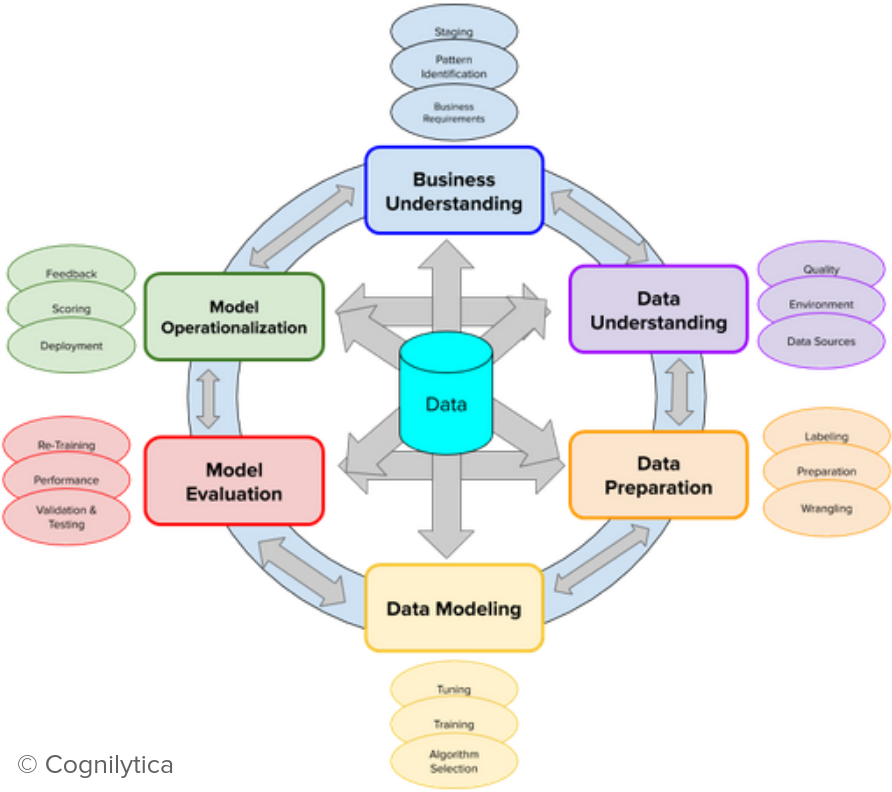
\includegraphics[width=0.4\textwidth]{figures/cpmai}
  \vspace{-4mm}
\caption{Das CPMAI-Prozess/Framework von Cognilytica}
\label{fig:cpmai}
\end{center}
\end{figure}

Diese Flexibilität und Übernahme moderner agiler Praktiken ermöglicht eine einfache Einbettung aktueller Entwicklungs-Best-Practices, z.\,B. Test-Driven Development (TDD). TDD ist eine test-first Softwareentwicklungs-Methodik, d.\,h. Tests werden geschrieben, bevor die eigentliche Software, d.\,h. das zu testende System (SUT), entwickelt wird. In TDD wird ein Rot-Grün-Refaktor-Zyklus befolgt: Ein neu geschriebener Test schlägt zunächst fehl, was die Aktualisierung des SUT motiviert, aber nur mit genug Entwicklung, um den neuen Test zu bestehen. Die neuen und alle alten Tests bieten ein Sicherheitsnetz, um Refactoring sowohl der Tests als auch des SUT zu ermöglichen. Schließlich können wir durch die nächste Schleife des Rot-Grün-Refaktor-Zyklus iterieren.

CPMAI kann leicht angepasst werden, um TDD einzubetten:
\begin{compactitem}
\item Die Data Preparation Phase ist die test-first Phase, in der ein fehlschlagender Test geschrieben wird
\item Die Data Modeling Phase ist die Entwicklungsphase, in der das SUT aktualisiert wird
\item Die Model Evaluation Phase ist die anschließende Testausführung. Wenn ein Test fehlschlägt oder wir das SUT refaktorieren wollen, gehen wir zurück zur Data Modeling Phase. Wenn wir einen weiteren Test hinzufügen oder Tests refaktorieren wollen, gehen wir zurück zur Data Preparation Phase.
\end{compactitem}

CPMAI kann auch das Guaranteed Safe AI Framework \cite{Dalrymple24} einbetten:
\begin{compactitem}
\item Die Data Preparation Phase aktualisiert die Sicherheitsspezifikation und das Weltmodell basierend auf den Erkenntnissen aus den Phasen Business Understanding und Data Understanding.
\item Die Data Modeling Phase wendet das Verifikationstool an, um das Modell zu evaluieren, idealerweise mit quantifizierbaren Sicherheitsgarantien.
\item Die Model Operationalization Phase setzt Laufzeit-Monitore ein, falls die Verifikation auch solche Überwachung abdecken soll.
\end{compactitem}

\subsection{Validieren von Produkt- und LLM-Eigenschaften}

Die Schleife von Model Operationalization zurück zu Business Understanding und Data Understanding in CPMAI ermöglicht häufiges Feedback von den Stakeholdern. Für MediVoice entwickelte Mediform ein Backend für Interaction Analytics auf anonymisierten Patientendialogen: Es bewertet Dialoge nach ihrer Länge, ihrem Autonomiegrad und ihren Kosten. Alle Dialoge werden nach der Absicht des Patienten und dem Versicherungstyp klassifiziert und aufgelistet, zusammen mit einer Zusammenfassung, für einen Drilldown, d.\,h. mit einem Link zu einer detaillierteren Ansicht zur weiteren Inspektion. Ihre Evaluierung (siehe Abb. \ref{fig:interactionanalytics}) hilft im Business Understanding, fehlerhafte oder nicht zufriedenstellende Dialoge zu finden. In der Data Understanding Phase führen wir Fehleranalysen durch, um Anwendungsfälle und Dialoge in Bezug auf Geschäftsanforderungen und Geschäftsprozesse zu verstehen und zu priorisieren. Die Ergebnisse der Fehleranalyse helfen in der Data Preparation Phase, die Trainings- und Testsätze zu aktualisieren und zu erweitern, indem Dialoge formuliert werden, die sich auf die hoch priorisierten Geschäftsanforderungen und Geschäftsprozesse konzentrieren. Somit werden alle in Mediforms CPMAI verwendeten Daten zu einer Form von (anonymisiertem) Patientendialog mit Metadaten vereinheitlicht: Ein Dialog, möglicherweise generalisiert durch das Enthalten einiger Template-Variablen, basierend auf dem gewünschten Gesprächsverhalten, das aus den anonymisierten Patientendialogen abgeleitet wurde. Die Trainings- und Testsätze decken eine breite Palette von Eingaben und erwarteten Ausgaben ab und sind entscheidend für die Evaluierung der Leistung des LLMs.

\begin{figure}[hbt!]
  \begin{center}
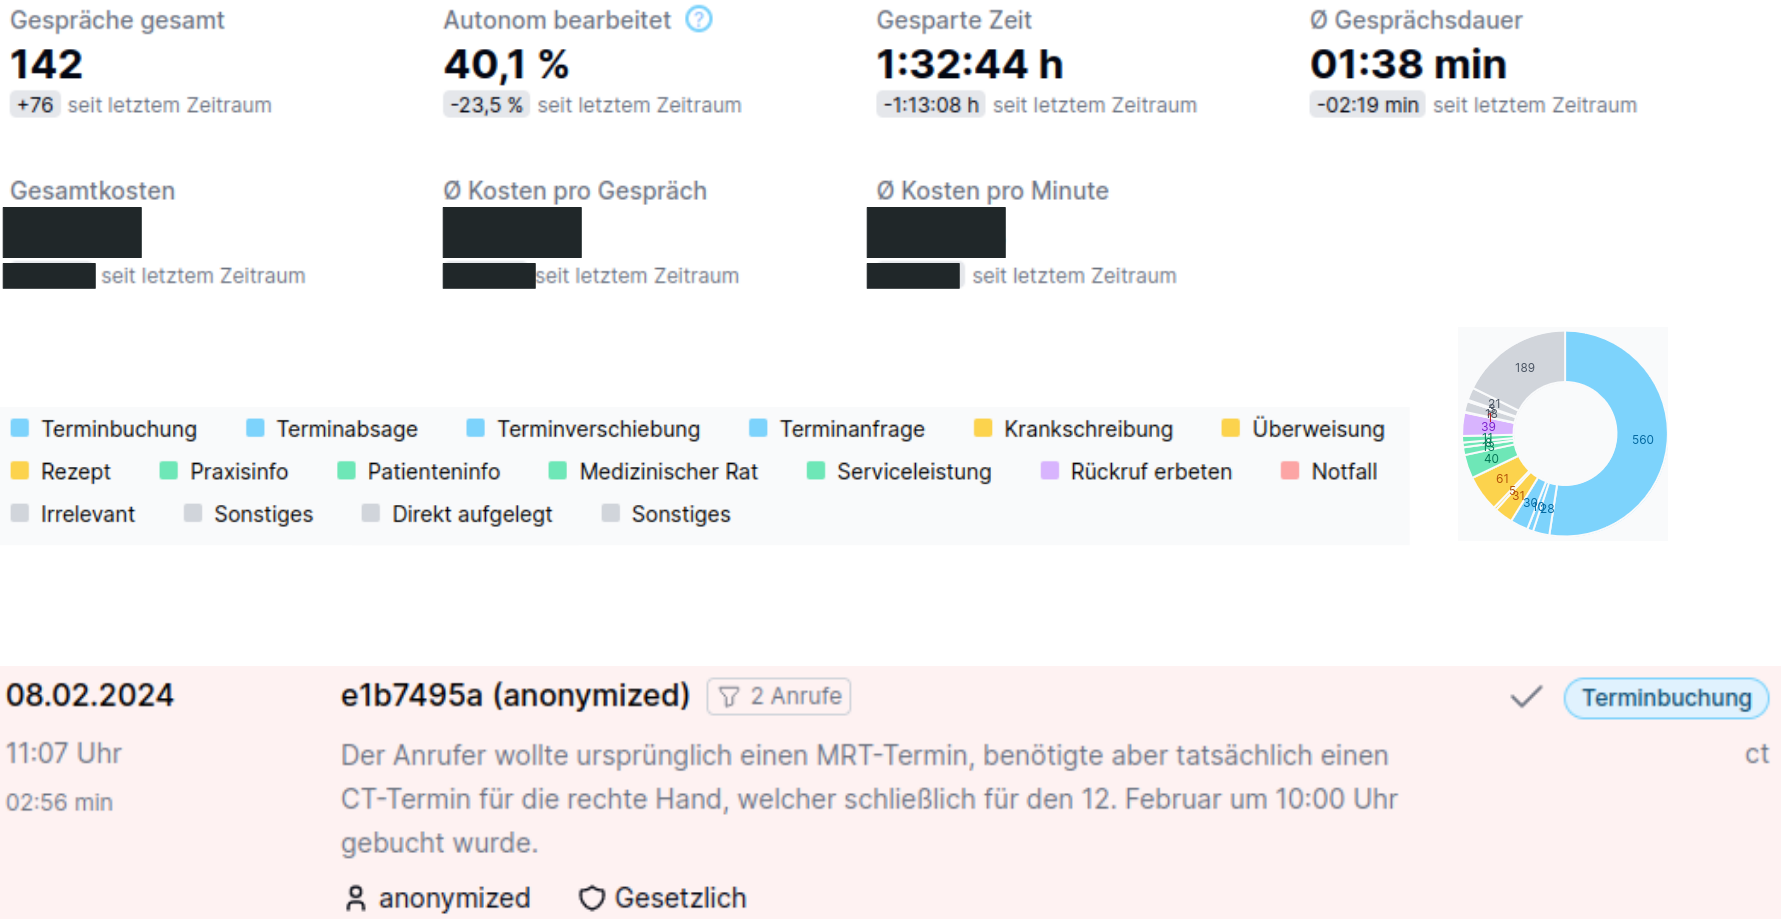
\includegraphics[width=0.5\textwidth]{figures/InteractionAnalytics}
  \vspace{-8mm}
\caption{Mediforms Interaction Analytics auf anonymisierten Patientendialogen}
\label{fig:interactionanalytics}
\end{center}
\end{figure}

Wir erweitern CPMAI um eine ATDD-Stil LLM-Entwicklung: Durch den oben beschriebenen Prozess sind die Dialoge oder Dialog-Templates innerhalb des Testsatzes geschäftszentriert und können als Akzeptanztests (ATs) betrachtet werden, d.\,h. als Tests, die auf kundenorientierte Weise basieren, basierend auf den Anforderungen des Kunden. Somit definieren ATs die Kriterien für die Akzeptanz der Software und stellen sicher, dass das Endprodukt die Bedürfnisse des Benutzers erfüllt. Durch die Verwendung eines TDD-ähnlichen Prozesses (siehe vorheriger Abschnitt) innerhalb unserer CPMAI-Iterationen erweitern wir CPMAI um eine ATDD-Stil LLM-Entwicklung, die zu \ATDLLMD{} führt. Im Gegensatz zu klassischem ATDD erfordert \ATDLLMD{} nicht, dass alle ATs bestehen, um das LLM insgesamt in Produktion zu akzeptieren, sondern dass ein Schwellenwert für eine Metrik wie Genauigkeit überschritten wird, wie es bei ML-Evaluierungen üblich ist. Wenn Kunden wissen, dass das LLM gegen kundenorientierte Testfälle mit einer geeigneten Metrik feinabgestimmt und getestet wurde, steigt auch ihr Vertrauen in das System.

\subsection{Verifizieren und Evaluieren von LLMs}

Um die Herausforderungen beim Verifizieren und Evaluieren von LLMs zu bewältigen, entwickeln wir unser eigenes neuartiges Testtool \textbf{LM-Eval}, das EleutherAIs Language Model Evaluation Harness \cite{Gao23} erweitert. EleutherAIs Tool ist hauptsächlich bekannt durch die Unterstützung von \cite{HF24}. Es enthält viele Benchmarks, Prompts und Metriken out of the box, bietet aber auch die Möglichkeit, sie zu erweitern und benutzerdefinierte Modelle zu evaluieren.

Für LM-Eval (siehe Abb.~\ref{fig:lmeval}) haben wir unter anderem hinzugefügt:
\begin{compactitem}
\item unseren eigenen Testtreiber, um die Testausführung natürlicher Dialoge in unserem eigenen Format zu ermöglichen, mit Template-Variablen und Metadaten, die Felder für Geschäftsprozesse enthalten können, die individuell für die betrachtete Arztpraxis sind
\item unsere eigenen geschäftszentrierten Testorakel und Metriken zur Evaluierung natürlicher Dialoge in Bezug auf natürliche Sprachverarbeitung und die Domäne. Zum Beispiel aggregieren wir statistisch, indem wir individuelle Ergebnisse basierend auf ihrer semantischen und geschäftlichen Relevanz gewichten (siehe Abb. \ref{fig:lmeval})
\item Funktionen zur Durchführung von nicht-deterministischem Black-Box-Testing. Zum Beispiel führen wir semantische Vergleiche durch (z.\,B. strenger für \texttt{pre} Anrufe als \texttt{msg} Anrufe, siehe Abb. \ref{fig:lmeval}) und erlauben die Angabe mehrerer alternativer Ausgaben.
\end{compactitem}
Mit unseren templatisierten Dialogtestsätzen als benutzerdefinierte Benchmarks kann LM-Eval unsere MediVoice-Modelle evaluieren und die in Abschnitt~\ref{sec:verifyandevaluatellms} beschriebenen Herausforderungen bewältigen.

Im Sinne des Guaranteed Safe AI Frameworks \cite{Dalrymple24} verwendet unser Testing mit LM-Eval
\begin{compactitem}
\item templatisierte Dialoge als Weltmodell, das zwischen Weltmodell-Level W0 und W1 liegt (auf einer Skala von W0 bis W5).
\item mehrere Assistenznachrichten in templatisierten Dialogen als Sicherheitsspezifikation, die auf Sicherheitsspezifikations-Level S3 liegt (auf einer Skala von S0 bis S7).
\item LM-Eval als Verifikator, der auf Verifikator-Level V2 für feste Template-Variablen-Substitutionen und auf Level V3 liegt, wenn die Substitution über vollständige Wertemengen randomisiert wird (auf einer Skala von V0 bis V10).
\end{compactitem}

Mediform verwendet ergänzende Testmethoden, die \ATDLLMD{} in einem Ensemble begleiten. Dies gibt weitere Einblicke und erhöht das Vertrauen. GS AI schlägt auch "Defence in Depth" vor, indem mehrere Schutzschichten eingesetzt werden, um gegen komplexe Bedrohungen zu verteidigen:

Eine zusätzliche Testmethode führt Smoke-Tests durch, bei denen ein bestimmtes Szenario und Patientenverhalten für ein LLM spezifiziert wird, um es zu interpretieren und gegen MediVoice auszuführen. Im Sinne von GS AI hat dies
\begin{compactitem}
\item ein LLM mit in-Kontext erlerntem Patientenverhalten als Weltmodell auf Level W1.
\item die spezifizierten Szenarien mit gewünschtem Kontrollfluss als Sicherheitsspezifikation auf Level S3.
\item das LLM, das die Verifikation nur auf die spezifizierten Szenarien fokussiert, was auf Level V2 ist.
\end{compactitem}

Mediform überwacht auch reale Patientendialoge (anonymisiert), mit einem Laufzeit-Monitor zur Halluzinationserkennung bzw. manuellen Inspektionen, um verbleibende Fehler und Erkenntnisse zu erfassen. Im Sinne von GS AI hat die Halluzinationserkennung
\begin{compactitem}
\item ein Halluzinationserkennungs-LLM auf Level W1 als Weltmodell
\item eine Spezifikation zu intrinsischer und extrinsischer Halluzination \cite{Ji23} als Sicherheitsspezifikation, die sich auf Widersprüche zwischen der Systemnachricht und dem Dialog konzentriert, was auf Level S2 ist
\item die Menge aller bisher anonymisierten realen Patientendialoge als standardisierter Testsatz, was auf Level V2 ist.
\end{compactitem}
Die manuellen Inspektionen haben Menschen mit ihrem Wissen und Annahmen als Weltmodell (Level W0) und Sicherheitsspezifikation (Level S1), wiederum auf allen bisher anonymisierten realen Patientendialogen (Level V2).

\begin{figure}[hbt!]
  \begin{center}
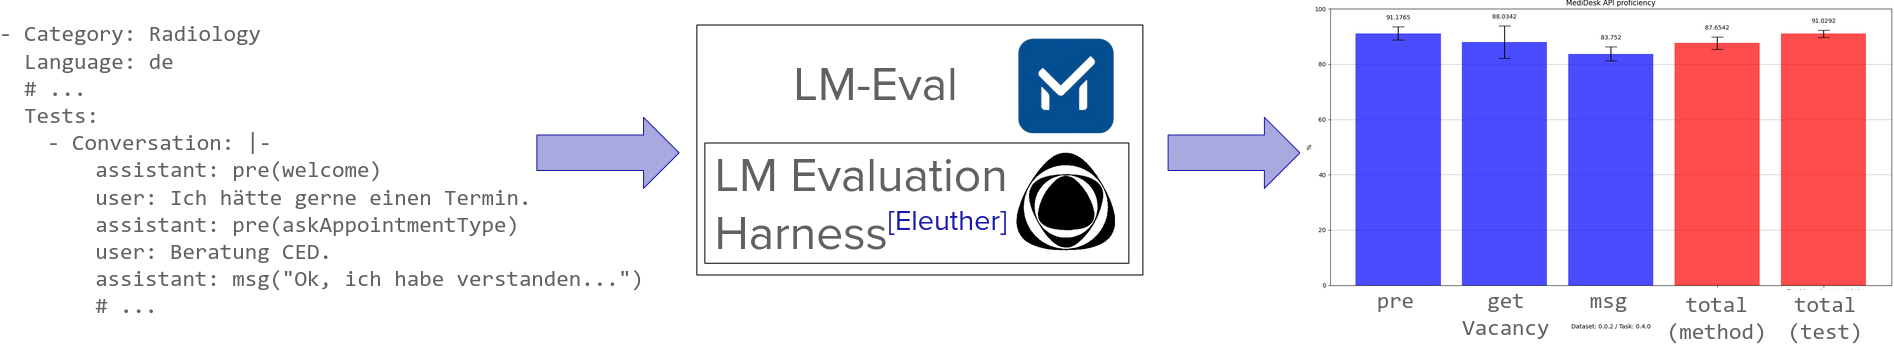
\includegraphics[width=0.5\textwidth]{figures/LMEval2}
  \vspace{-8mm}
\caption{Mediforms LM-Eval Testing Framework}
\label{fig:lmeval}
\end{center}
\end{figure}

\subsection{Kombinieren aller Lösungen}

Mit CPMAI und LM-Eval an Ort und Stelle können wir eine CPMAI-Rundreise mit \ATDLLMD{} durchführen: Wir sammeln iterativ Dialoge von realen Patienten in der Model Operationalization Phase, d.\,h. die Interaktionen der Patienten mit unserem neuartigen Telefon-Bot. Wir anonymisieren sie in einer DSGVO-konformen Weise und führen dann Business und Data Understanding darauf durch, mit Hilfe unseres Interaction Analytics Dashboards sowie manueller Exploration. Anhand der gesammelten Dialoge, insbesondere derjenigen mit unerwünschtem Verhalten, und Erkenntnissen aus Fehleranalysen darüber, aktualisieren wir Dialoge und möglicherweise die Weltmodelle und Sicherheitsspezifikationen und erstellen in der Data Preparation Phase neue Dialoge mit dem entsprechenden gewünschten Verhalten. Die Dialoge werden als Trainingsdaten oder Akzeptanztests spezifiziert, die die aktuelle CPMAI-Iteration von Rot (fehlschlagende Akzeptanztests) während der Data Preparation, über Data Modeling (Training), zu Grün (bestehende Akzeptanztests) während Model Evaluation und Operationalization treiben. Testausführung und Evaluierung werden von LM-Eval und ergänzenden Testmethoden durchgeführt. Im Gegensatz zu klassischem ATDD müssen nicht alle Akzeptanztests grün werden, sondern nur genug, um die geforderte Metrik zu erreichen, z.\,B. 90\,\% Genauigkeit. Dieser \textbf{Rot-Train-Grün-Zyklus} in \ATDLLMD{} ähnelt ATDD, integriert aber Data-Science-Best-Practices. Er ähnelt auch CPMAI, integriert aber weitere moderne Softwareentwicklung, Testing und Safety Engineering Best Practices.

\section{Schlussfolgerung}

Zusammenfassend stellt die Anwendung von ATDD auf das Fine-Tuning von LLMs einen bedeutenden Schritt nach vorne bei der Entwicklung zuverlässigerer, genauerer und benutzerzentrierter AI-Sprachsysteme dar. Dieser \ATDLLMD{}-Ansatz verbessert nicht nur die Qualität der Ausgaben, sondern stärkt auch das Vertrauen der Benutzer in AI-Technologien.

Obwohl unsere Anwendung ASL-1 ist, geben wir Sicherheitsgarantien mit einem Ensemble von Testmethoden, mit Weltmodellen bis Level W1, Sicherheitsspezifikation bis Level S3 und Verifikatoren bis Level V3.

Als zukünftige Arbeit untersuchen wir Möglichkeiten, Teile dieses Prozesses zu automatisieren, indem wir AI selbst verwenden, um Test-Szenarien und Spezifikationen zu generieren und zu aktualisieren. Darüber hinaus versuchen wir, Feedback von verschiedenen Benutzern direkt in unser Modell zu integrieren (anstatt Feedback selbst abzuleiten und das Feedback zu verwenden, um neue Test- und Trainingsdaten manuell abzuleiten).

\section{Danksagungen}

Dank geht an Jochen Krause, CEO der Mediform GmbH, für die Möglichkeit, an dieser interessanten Aufgabe zu arbeiten, und an meine Kollegen für die großartige Arbeitsumgebung.

Dank geht an Cognilytica, LLC, die das Urheberrecht und die Marke für die CPMAI-Methodik und Bilder besitzen (Verwendung hier mit schriftlicher Genehmigung).

\section{Bibliographie}

\small
\begin{thebibliography}{99}
\bibitem{Akiba24} Akiba, Takuya, et al. "Evolutionary optimization of model merging recipes." arXiv preprint arXiv:2403.13187. 2024.

\bibitem{Brown20} Brown, Tom, et al. "Language models are few-shot learners." Advances in neural information processing systems 33. 2020.

\bibitem{Chang24} Chang, Yupeng, et al. "A survey on evaluation of large language models." ACM Transactions on Intelligent Systems and Technology 15.3 (2024): 1--45.

\bibitem{Cognilytica} Cognilytica. “The Seven Patterns of AI”. \url{https://www.cognilytica.com/the-seven-patterns-of-ai/}

\bibitem{CPMAI} Cognilytica: “Cognitive Project Management For AI”, \url{https://www.cognilytica.com/what-is-the-cognitive-project-management-for-ai-cpmai-methodology/}

\bibitem{CRISP99} “Cross Industry Standard Process for Data Mining 1.0”. \url{https://web.archive.org/web/20220401041957/https://www.the-modeling-agency.com/crisp-dm.pdf}

\bibitem{Dettmers22} Dettmers, T., Lewis, M., Belkada, Y., and Zettlemoyer, L. "LLM.int8(): 8-bit matrix multiplication for transformers at scale." Advances in Neural Information Processing Systems 35. 2022.

\bibitem{Farago23} Faragó, David. "Engineering A Reliable Prompt For Generating Unit Tests -- Prompt engineering for QA \& QA for prompt engineering." Softwaretechnik-Trends (STT) 43(3). 2023.

\bibitem{Gao23} Gao, Leo, et al. “A framework for few-shot language model evaluation." 2023. \url{https://zenodo.org/records/10256836}

\bibitem{Github23} Github. “How to build an enterprise LLM application: Lessons from GitHub Copilot”. \url{https://github.blog/2023-09-06-how-to-build-an-enterprise-llm-application-lessons-from-github-copilot/}.

\bibitem{Gra23} Gramener Blog: "Large Language Models (LLMs): A Technology Gifted by Aliens Without a Manual". 2023. \url{https://blog.gramener.com/large-language-models-llms-technology}

\bibitem{HF24} Hugging Face. "Open LLM Leaderboard". 2024. \url{https://huggingface.co/spaces/HuggingFaceH4/open_llm_leaderboard}

\bibitem{Hosseini20} Hosseini-Asl, Ehsan, et al. "A simple language model for task-oriented dialogue." Advances in Neural Information Processing Systems 33. 2020.

\bibitem{Kaplan20} Kaplan, Jared, et al. "Scaling laws for neural language models." arXiv preprint arXiv:2001.08361. 2020.

\bibitem{Ke23} Ke, Zixuan, et al. "Continual pre-training of language models." arXiv preprint arXiv:2302.03241. 2023.

\bibitem{Liu22} Liu, Haokun, et al. "Few-shot parameter-efficient fine-tuning is better and cheaper than in-context learning." Advances in Neural Information Processing Systems 35. 2022.

\bibitem{Mediform24} Mediform: “Ältere Menschen buchen problemlos Termine via MediVoice”. \url{https://tinyurl.com/medivoice}.

\bibitem{MediVoice} Mediform. “Die Revolution für das Praxistelefon”. \url{https://mediform.io/medivoice/}

\bibitem{Minaee24} Minaee, Shervin, et al. "Large language models: A survey." arXiv preprint arXiv:2402.06196. 2024.

\bibitem{Röttger24} Röttger, Nils, Gerhard Runze, and Verena Dietrich. \emph{Basiswissen KI-Testen: Qualität von und mit KI-basierten Systemen: Aus- und Weiterbildung zum Certified Tester AI Testing: Foundation Level Specialist nach ISTQB®-Standard}. punkt.verlag. 2024.

\bibitem{Studer21} Studer, Stefan, et al. "Towards CRISP-ML (Q): a machine learning process model with quality assurance methodology." Machine learning and knowledge extraction 3.2. 2021.

\bibitem{Vaswani17} Vaswani, Ashish, et al. "Attention is all you need." Advances in neural information processing systems 30. 2017.

\bibitem{Wang24} Chen, Wang, et al. "Systems engineering issues for industry applications of large language model." Applied Soft Computing 151. 2024.

\end{thebibliography}

\end{document}
